\documentclass[border=5pt]{standalone}
\usepackage{amsmath}
\usepackage{tikz}
\usetikzlibrary{arrows.meta,positioning,shapes.geometric}
\usepackage{times}

\begin{document}
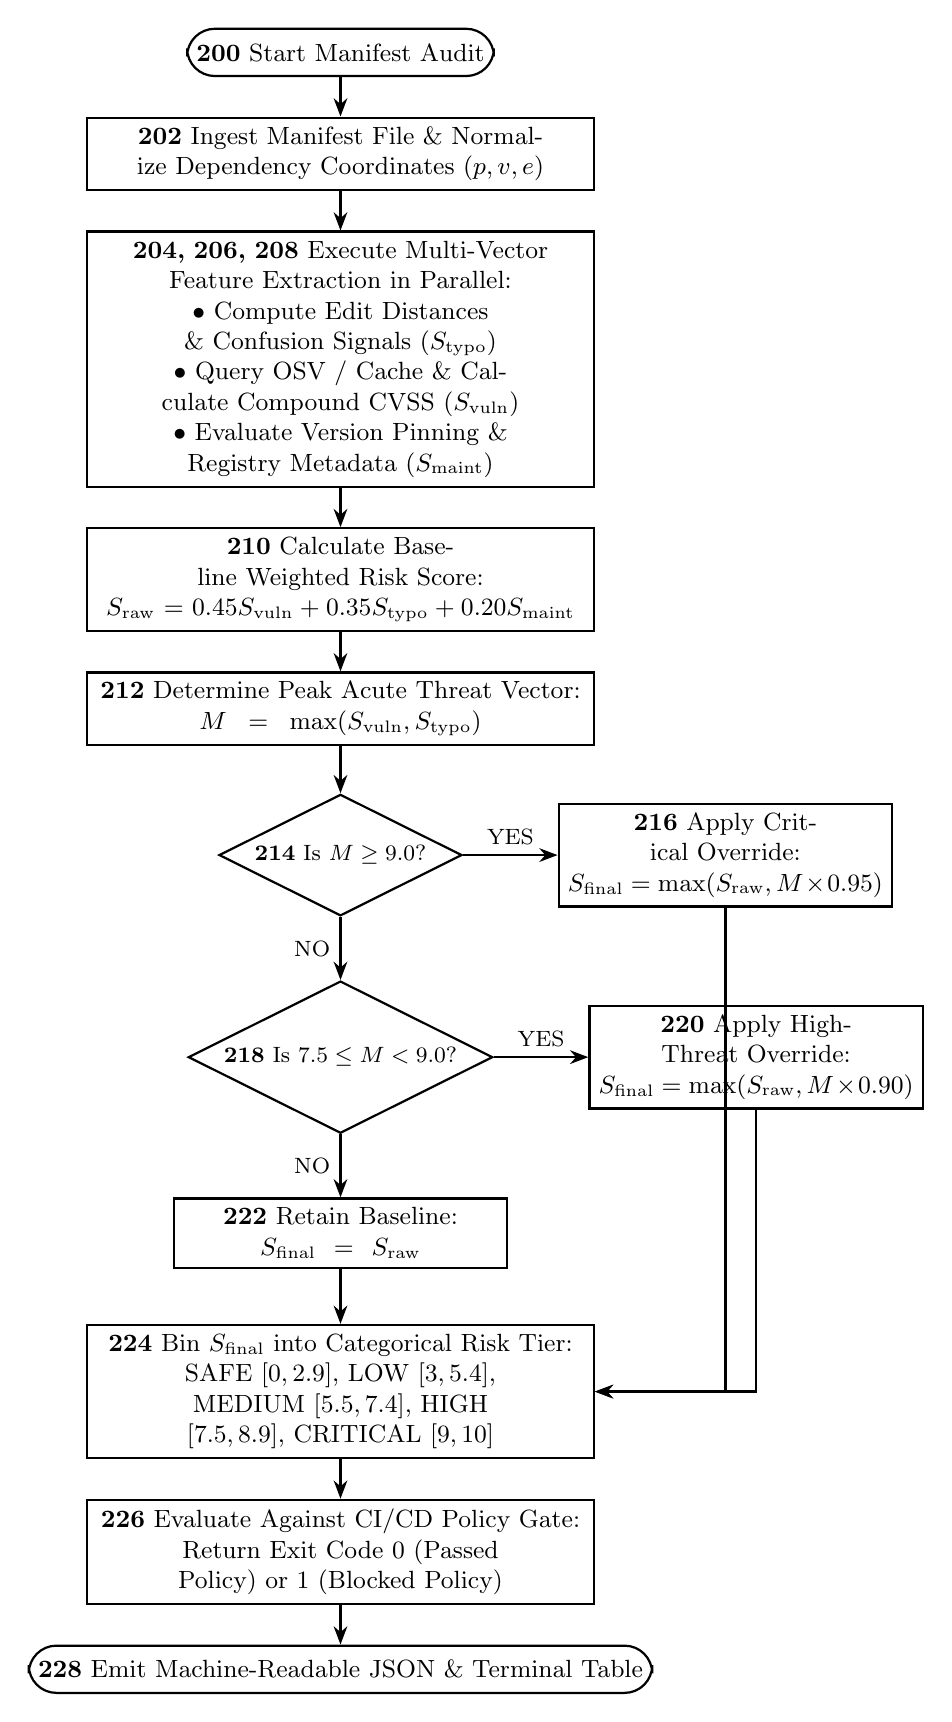
\begin{tikzpicture}[
    node distance=0.8cm and 0.8cm,
    startstop/.style={rectangle, rounded corners=10pt, draw=black, thick, fill=white, minimum height=0.6cm, align=center, font=\small},
    process/.style={rectangle, draw=black, thick, fill=white, minimum height=0.65cm, align=center, font=\small, text width=6.2cm},
    decision/.style={diamond, draw=black, thick, fill=white, aspect=2.0, align=center, font=\footnotesize, inner sep=2pt},
    arrow/.style={-{Stealth[scale=1.0]}, thick, draw=black}
]

\node[startstop] (start) {\textbf{200} Start Manifest Audit};
\node[process, below=0.5cm of start] (ingest) {\textbf{202} Ingest Manifest File \& Normalize Dependency Coordinates $(p, v, e)$};
\draw[arrow] (start) -- (ingest);

\node[process, below=0.5cm of ingest] (parallel) {\textbf{204, 206, 208} Execute Multi-Vector Feature Extraction in Parallel:\\
$\bullet$ Compute Edit Distances \& Confusion Signals ($S_{\text{typo}}$)\\
$\bullet$ Query OSV / Cache \& Calculate Compound CVSS ($S_{\text{vuln}}$)\\
$\bullet$ Evaluate Version Pinning \& Registry Metadata ($S_{\text{maint}}$)};
\draw[arrow] (ingest) -- (parallel);

\node[process, below=0.5cm of parallel] (raw) {\textbf{210} Calculate Baseline Weighted Risk Score:\\
$S_{\text{raw}} = 0.45 S_{\text{vuln}} + 0.35 S_{\text{typo}} + 0.20 S_{\text{maint}}$};
\draw[arrow] (parallel) -- (raw);

\node[process, below=0.5cm of raw] (maxvec) {\textbf{212} Determine Peak Acute Threat Vector:\\
$M = \max(S_{\text{vuln}}, S_{\text{typo}})$};
\draw[arrow] (raw) -- (maxvec);

\node[decision, below=0.6cm of maxvec] (d1) {\textbf{214} Is $M \ge 9.0$?};
\draw[arrow] (maxvec) -- (d1);

\node[process, right=1.2cm of d1, text width=4.0cm] (crit) {\textbf{216} Apply Critical Override:\\
$S_{\text{final}} = \max(S_{\text{raw}}, M \times 0.95)$};
\draw[arrow] (d1) -- node[above, font=\footnotesize] {YES} (crit);

\node[decision, below=0.8cm of d1] (d2) {\textbf{218} Is $7.5 \le M < 9.0$?};
\draw[arrow] (d1) -- node[left, font=\footnotesize] {NO} (d2);

\node[process, right=1.2cm of d2, text width=4.0cm] (high) {\textbf{220} Apply High-Threat Override:\\
$S_{\text{final}} = \max(S_{\text{raw}}, M \times 0.90)$};
\draw[arrow] (d2) -- node[above, font=\footnotesize] {YES} (high);

\node[process, below=0.8cm of d2, text width=4.0cm] (norule) {\textbf{222} Retain Baseline:\\
$S_{\text{final}} = S_{\text{raw}}$};
\draw[arrow] (d2) -- node[left, font=\footnotesize] {NO} (norule);

\node[process, below=0.7cm of norule, text width=6.2cm] (bin) {\textbf{224} Bin $S_{\text{final}}$ into Categorical Risk Tier:\\
SAFE $[0, 2.9]$, LOW $[3, 5.4]$, MEDIUM $[5.5, 7.4]$, HIGH $[7.5, 8.9]$, CRITICAL $[9, 10]$};
\draw[arrow] (norule) -- (bin);
\draw[arrow] (crit) |- (bin);
\draw[arrow] (high) |- (bin);

\node[process, below=0.5cm of bin] (gate) {\textbf{226} Evaluate Against CI/CD Policy Gate:\\
Return Exit Code 0 (Passed Policy) or 1 (Blocked Policy)};
\draw[arrow] (bin) -- (gate);

\node[startstop, below=0.5cm of gate] (end) {\textbf{228} Emit Machine-Readable JSON \& Terminal Table};
\draw[arrow] (gate) -- (end);

\end{tikzpicture}
\end{document}
